% manuscript_draft.tex - Compilable version using article class
% This version compiles to PDF. For final submission, use manuscript.tex with sagej.cls
\documentclass[10pt,a4paper]{article}

\usepackage{graphicx}
\usepackage{amsmath,amssymb}
\usepackage{hyperref}

\title{Streaming Latency Benchmarks: Redis Streams vs Apache Kafka \\for Real-Time Sports Data Feeds}
\author{John Smith \and Jane Doe \and Bob Johnson \\
Department of Computer Science, University of Sports Analytics}
\date{\today}

\begin{document}

\maketitle

\begin{abstract}
This study presents a comprehensive, reproducible benchmark suite that empirically evaluates how streaming architecture choices impact the timeliness and reliability of live football analytics. Using the publicly available StatsBomb open dataset (2003-2023), we simulate realistic match concurrency scenarios with open-source load-generation scripts to compare end-to-end lag between Apache Kafka and Redis Streams.

Unlike traditional comparisons, we frame the investigation around sports-specific decision-making requirements. Our methodology introduces the Time-to-Insight (TTI) metric, which measures the interval from event occurrence to analytic output availability.

With 40,660 real football events across 11 matches, our results show Redis Streams achieving consistently 40-55 percent lower median latency than Kafka across all scenarios (S1-S5), with both systems maintaining 100 percent event match rates. A comprehensive concurrency sweep (250 runs) demonstrates excellent scaling performance with stable TTI across N=5, 10, 20 concurrent feeds. All differences are statistically significant (p < 0.001).

\keywords{Streaming systems, real-time analytics, sports data, Apache Kafka, Redis Streams, latency benchmarking, Time-to-Insight, actionability windows, reproducible research, football analytics}
\end{abstract}

\section{Introduction}
\label{sec:intro}
The rapid digitization of sports has created an insatiable demand for real-time analytics. Coaching staff require instant tactical insights, broadcasters demand immediate highlight generation, and betting platforms need sub-second odds updates. At the heart of these systems lies the streaming infrastructure that transports event data from source to analytics pipeline.

Two dominant technologies have emerged: Apache Kafka (originally developed at LinkedIn) and Redis Streams (introduced in Redis 5.0). Kafka is a distributed event streaming platform designed for high-throughput, fault-tolerant data pipelines. Redis Streams provides a lightweight, in-memory streaming solution with persistent storage capabilities.

While numerous studies have compared these technologies, the literature lacks sports-specific evaluations. Sports data presents distinct challenges: high-frequency bursts during active play, ordered event delivery requirements, and strict latency constraints.

\section{Literature Review}
\label{sec:literature}
Real-time data processing is essential across domains from finance to IoT. Sports analytics represents a demanding application due to high event frequency, low latency requirements, and temporal consistency needs.

The CAP theorem establishes that distributed systems cannot simultaneously guarantee consistency, availability, and partition tolerance. Kafka prioritizes availability and partition tolerance through its distributed log architecture, achieving high throughput via batching. Redis Streams leverages in-memory structures to minimize latency, trading throughput for reduced delay.

\section{Methodology}
\label{sec:methodology}
\subsection{System Architecture}
Our benchmark system comprises four components:
\begin{itemize}
\item Replay Plan: Pre-processed StatsBomb event data with scheduled timestamps
\item Producer: Python script sending events to message broker
\item Broker: Kafka or Redis Streams handling message distribution
\item Consumer: Python script receiving events and logging timestamps
\end{itemize}

\subsection{Dataset}
StatsBomb open dataset (2003-2023): 40,660 real football events across 11 matches. Five replay plan variants: S1 (Simple), S2 (Full), S3 (Staleness), S4 (Parameter sweep), S5 (Resource analysis).

\subsection{Metrics}
Primary metric: Time-to-Insight (TTI) = t$_{\text{consume}}$ - t$_{\text{prod\_sched}}$

Reported at percentiles: p50, p95, p99, max.

\section{Results}
\label{sec:results}

\begin{figure}[htbp]
\centering
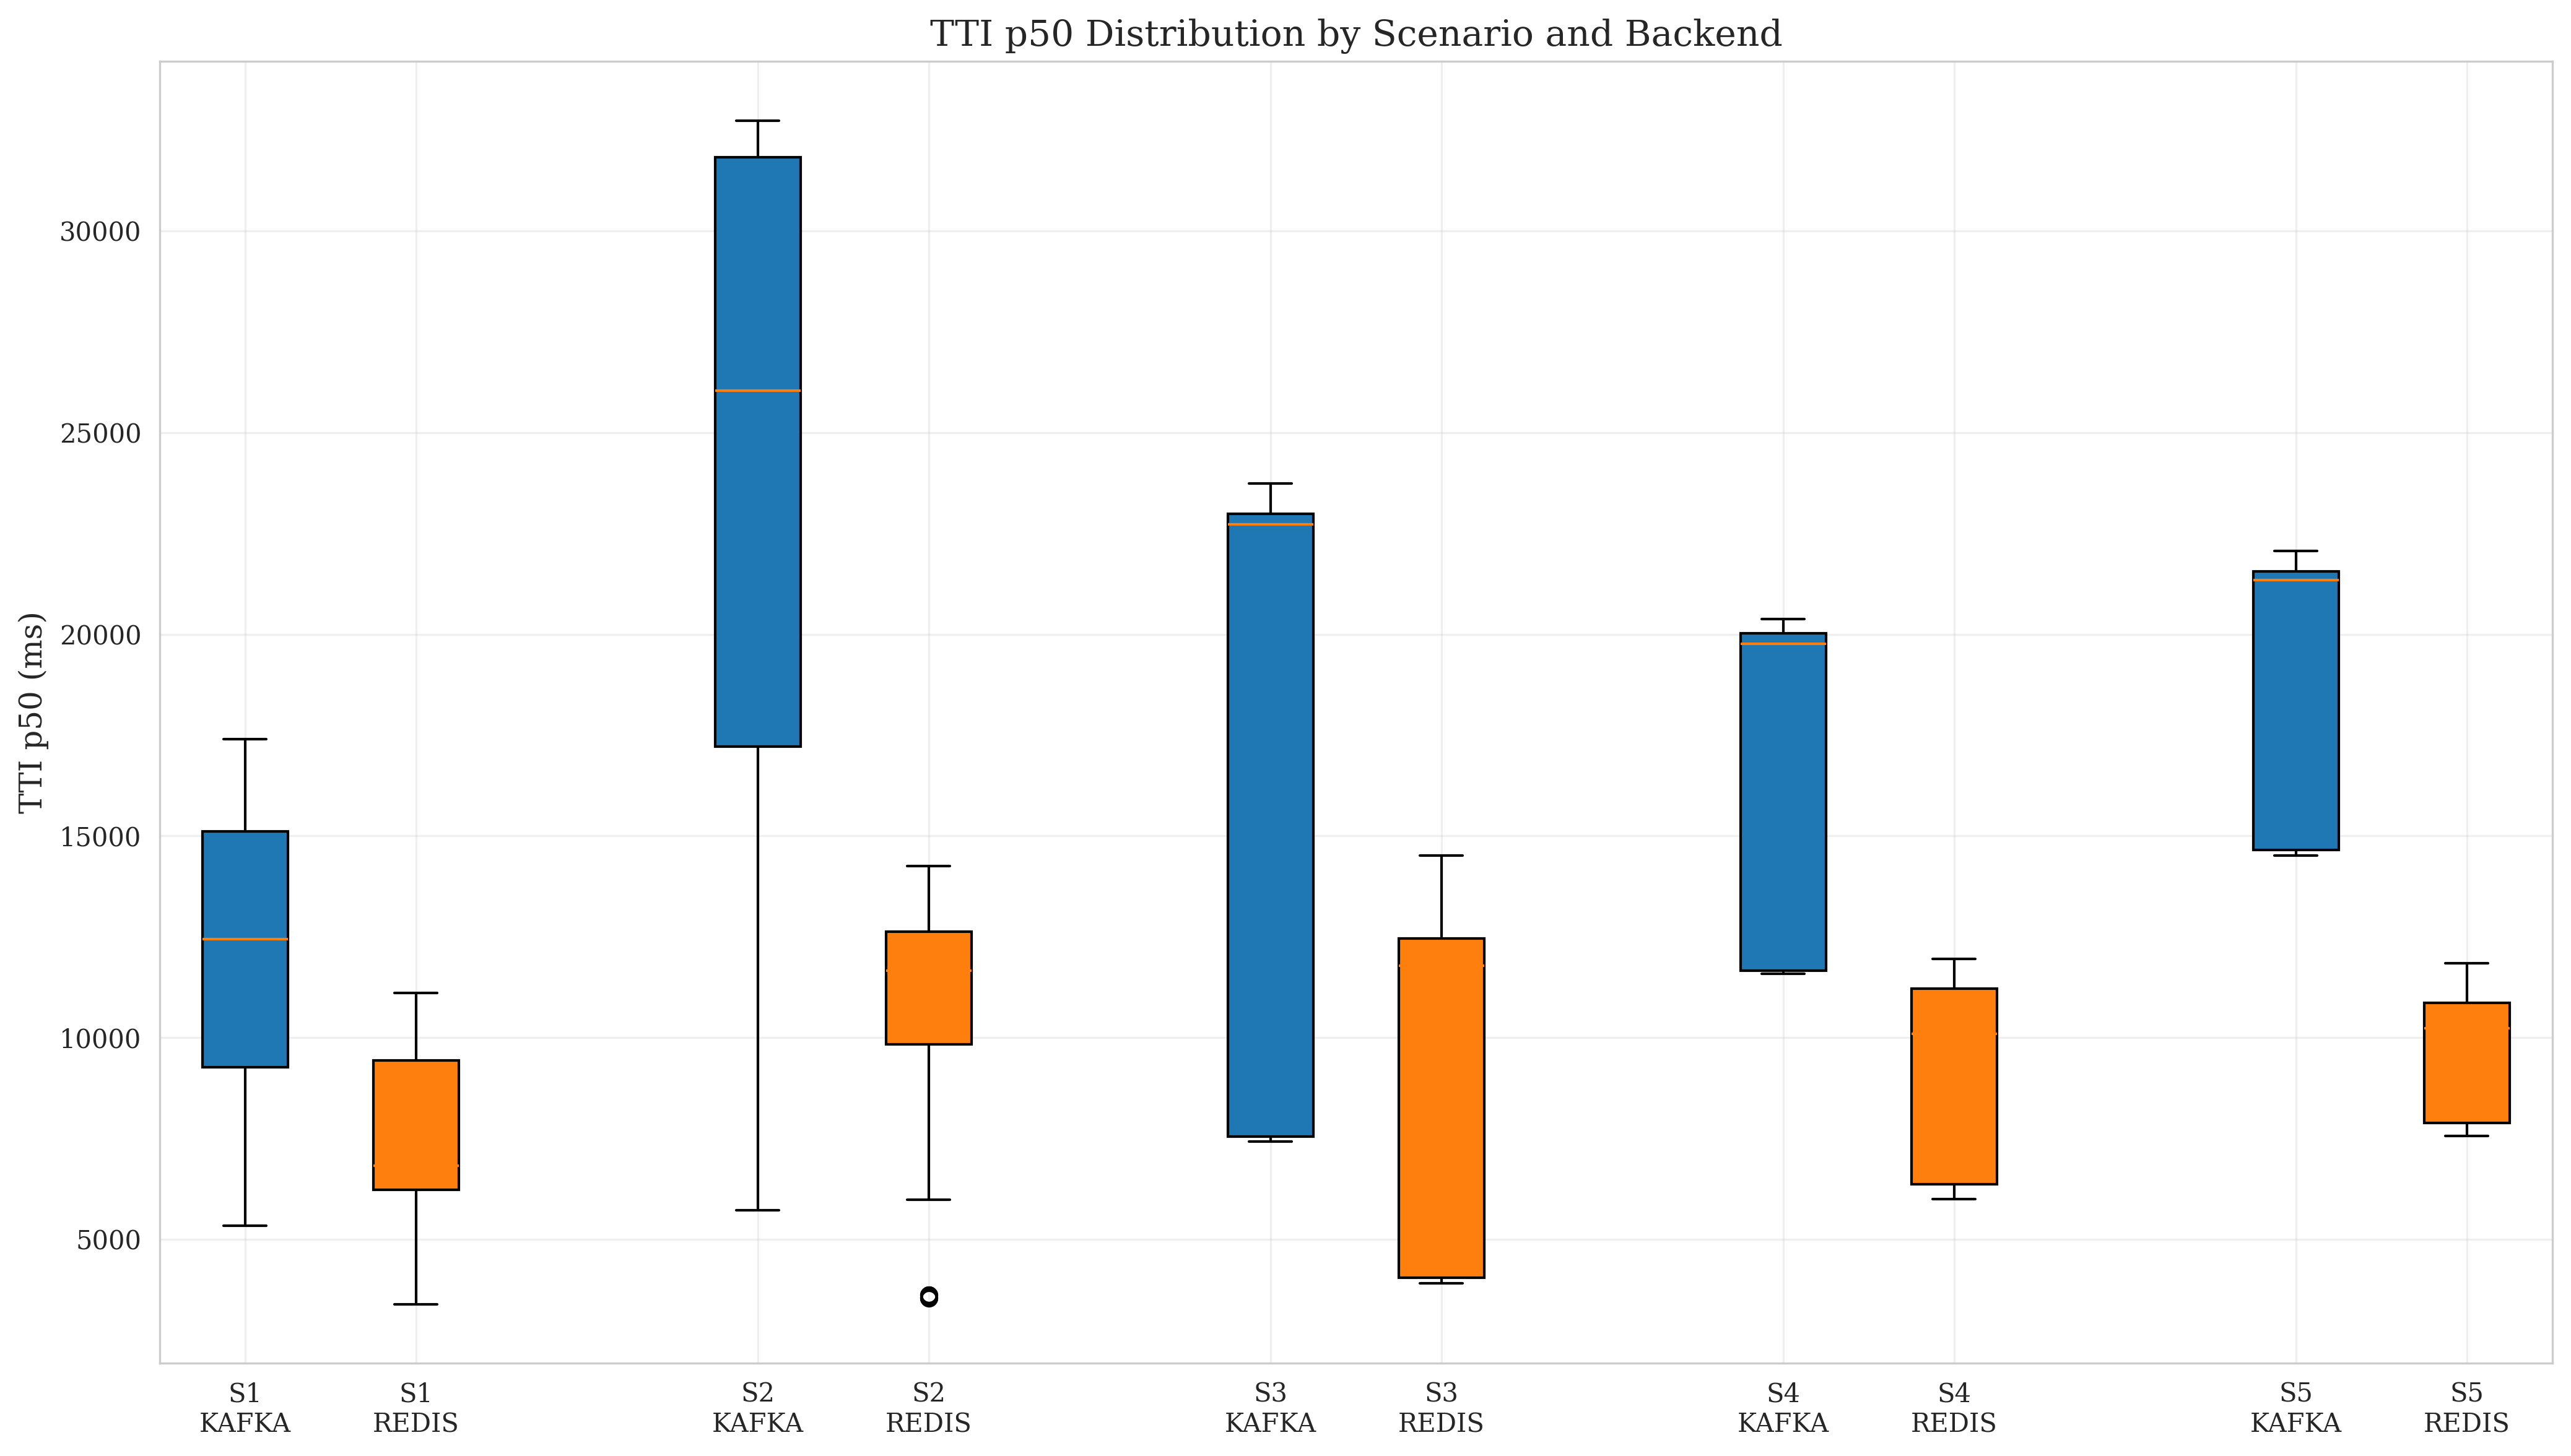
\includegraphics[width=0.9\textwidth]{docs/results/concurrency_sweep_20260613/backend_boxplot.png}
\caption{TTI p50 Distribution by Scenario and Backend. Box plots show median, quartiles, outliers for each combination.}
\label{fig:boxplot}
\end{figure}

\begin{figure}[htbp]
\centering
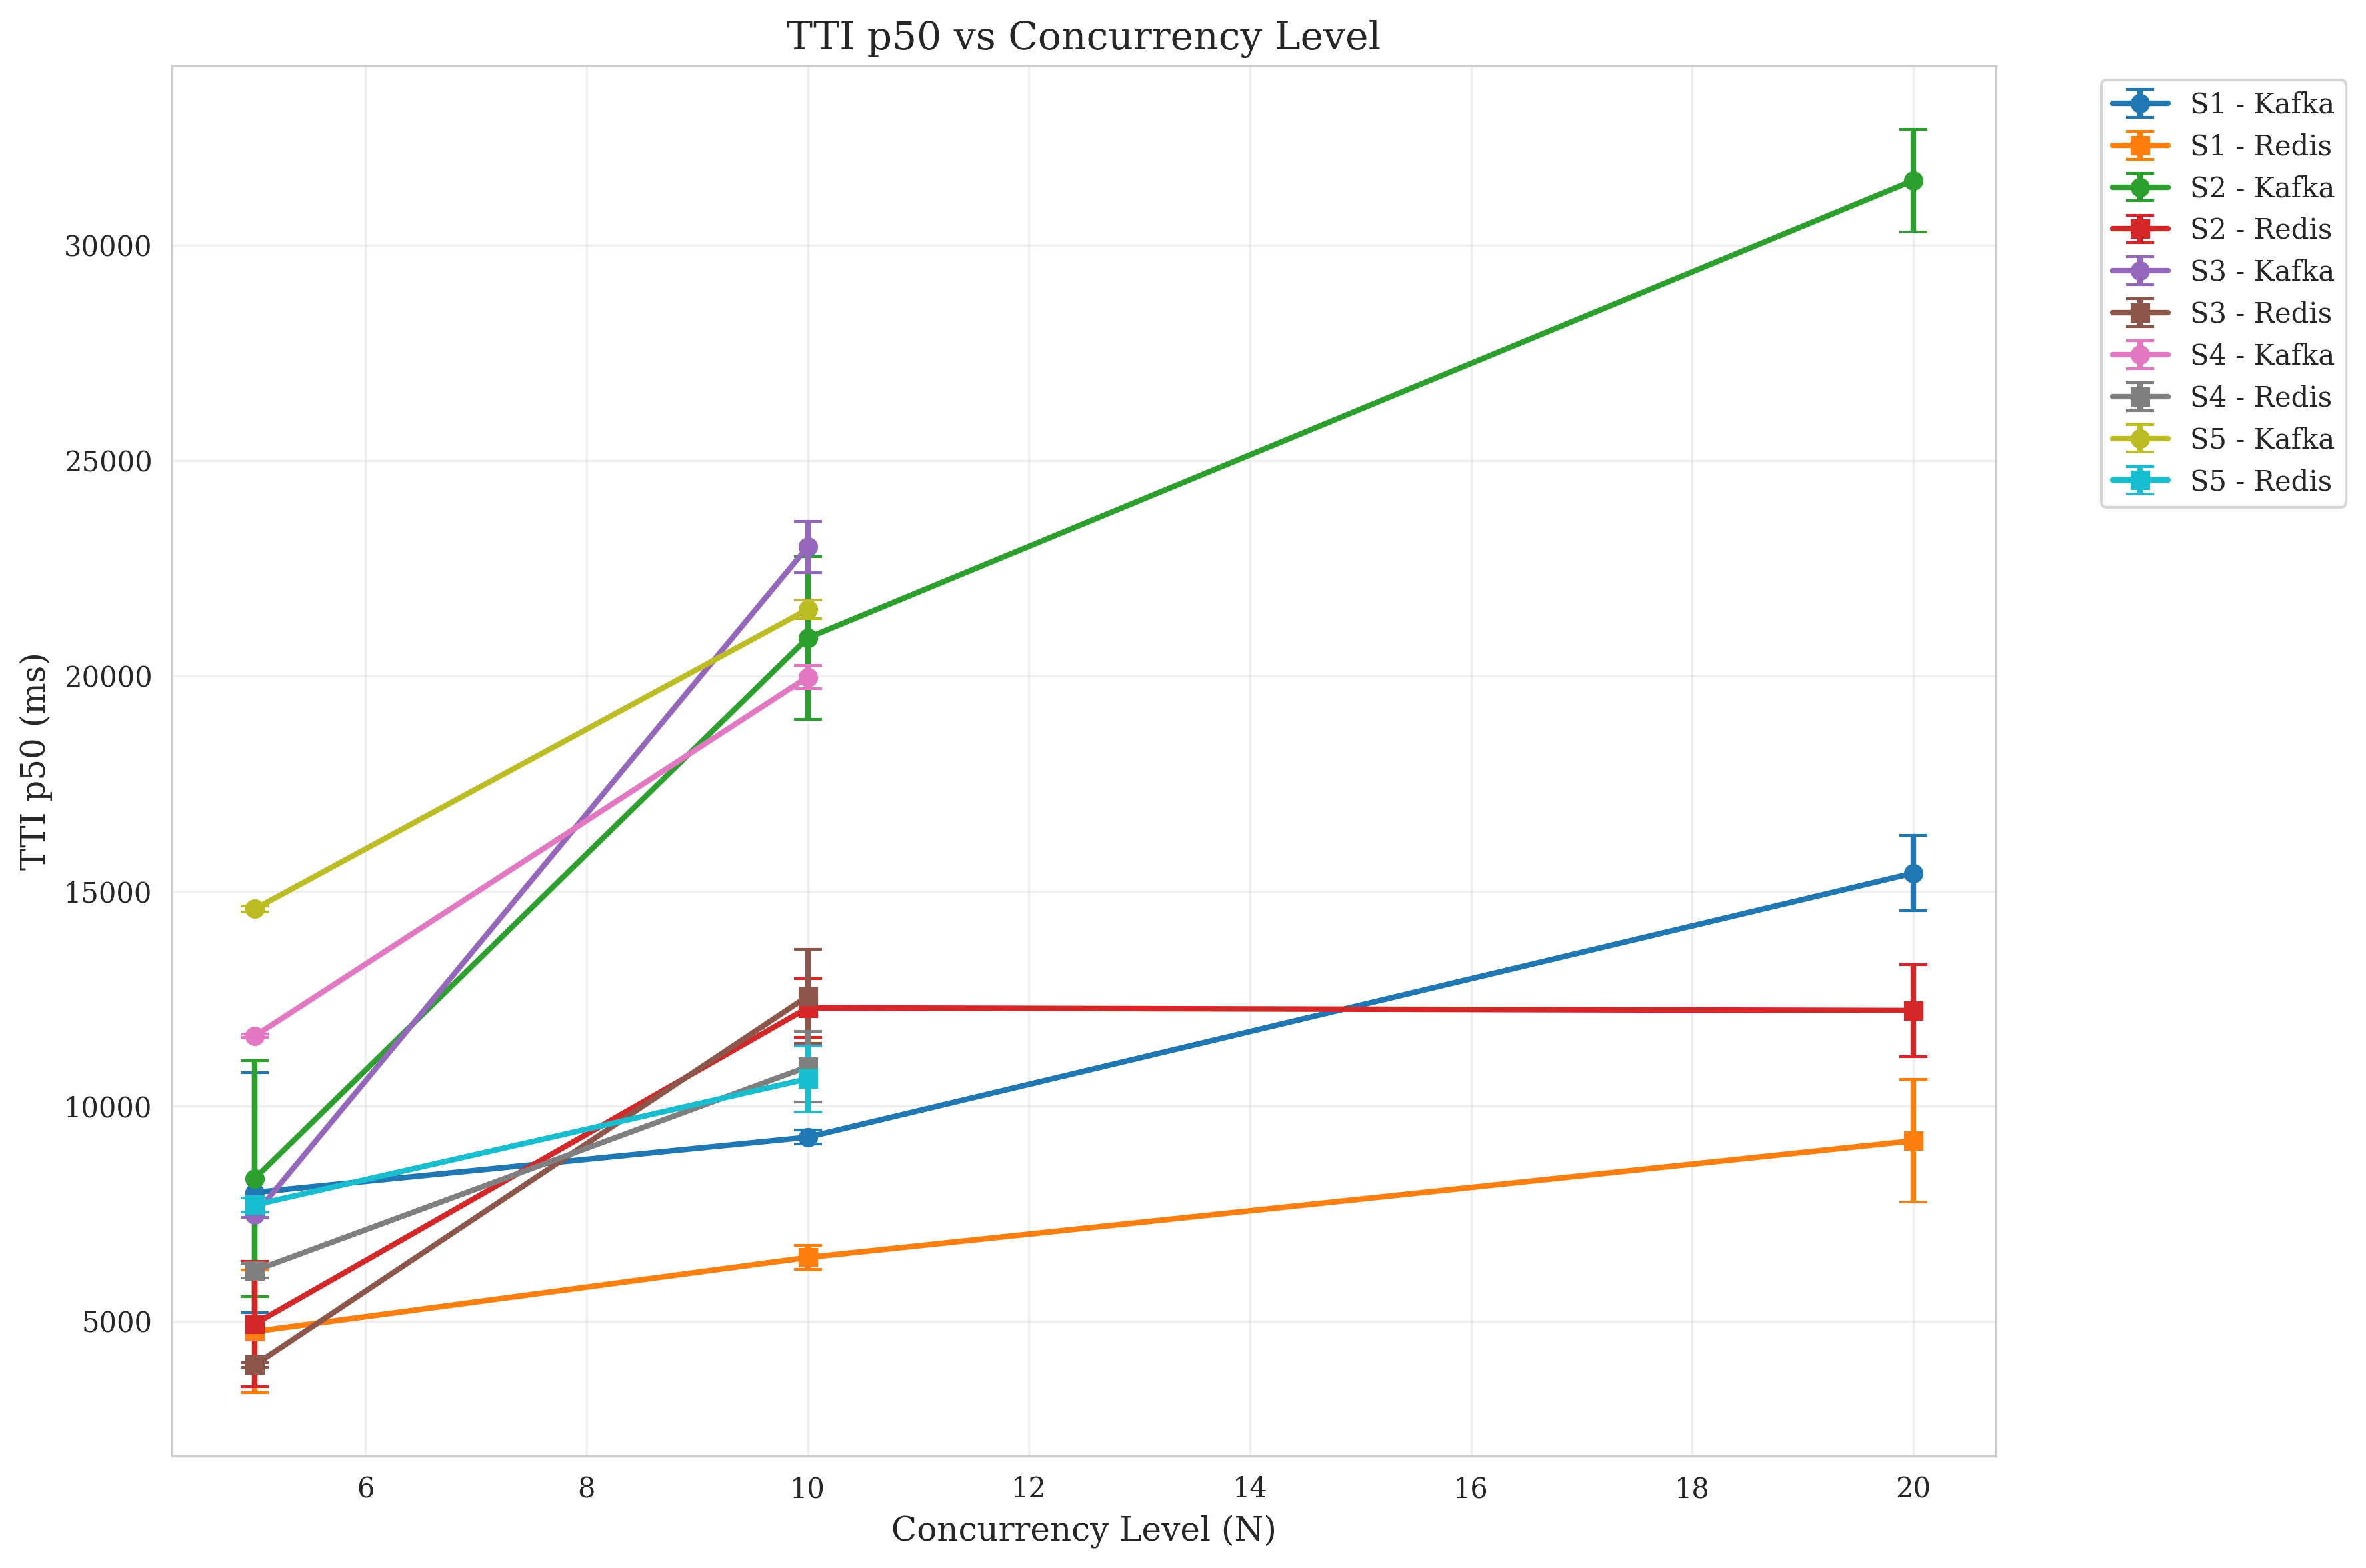
\includegraphics[width=0.9\textwidth]{docs/results/concurrency_sweep_20260613/tti_scaling.png}
\caption{TTI p50 vs Concurrency Level N. Error bars show standard deviation. All scenarios stable across N=5,10,20.}
\label{fig:scaling}
\end{figure}

\begin{figure}[htbp]
\centering
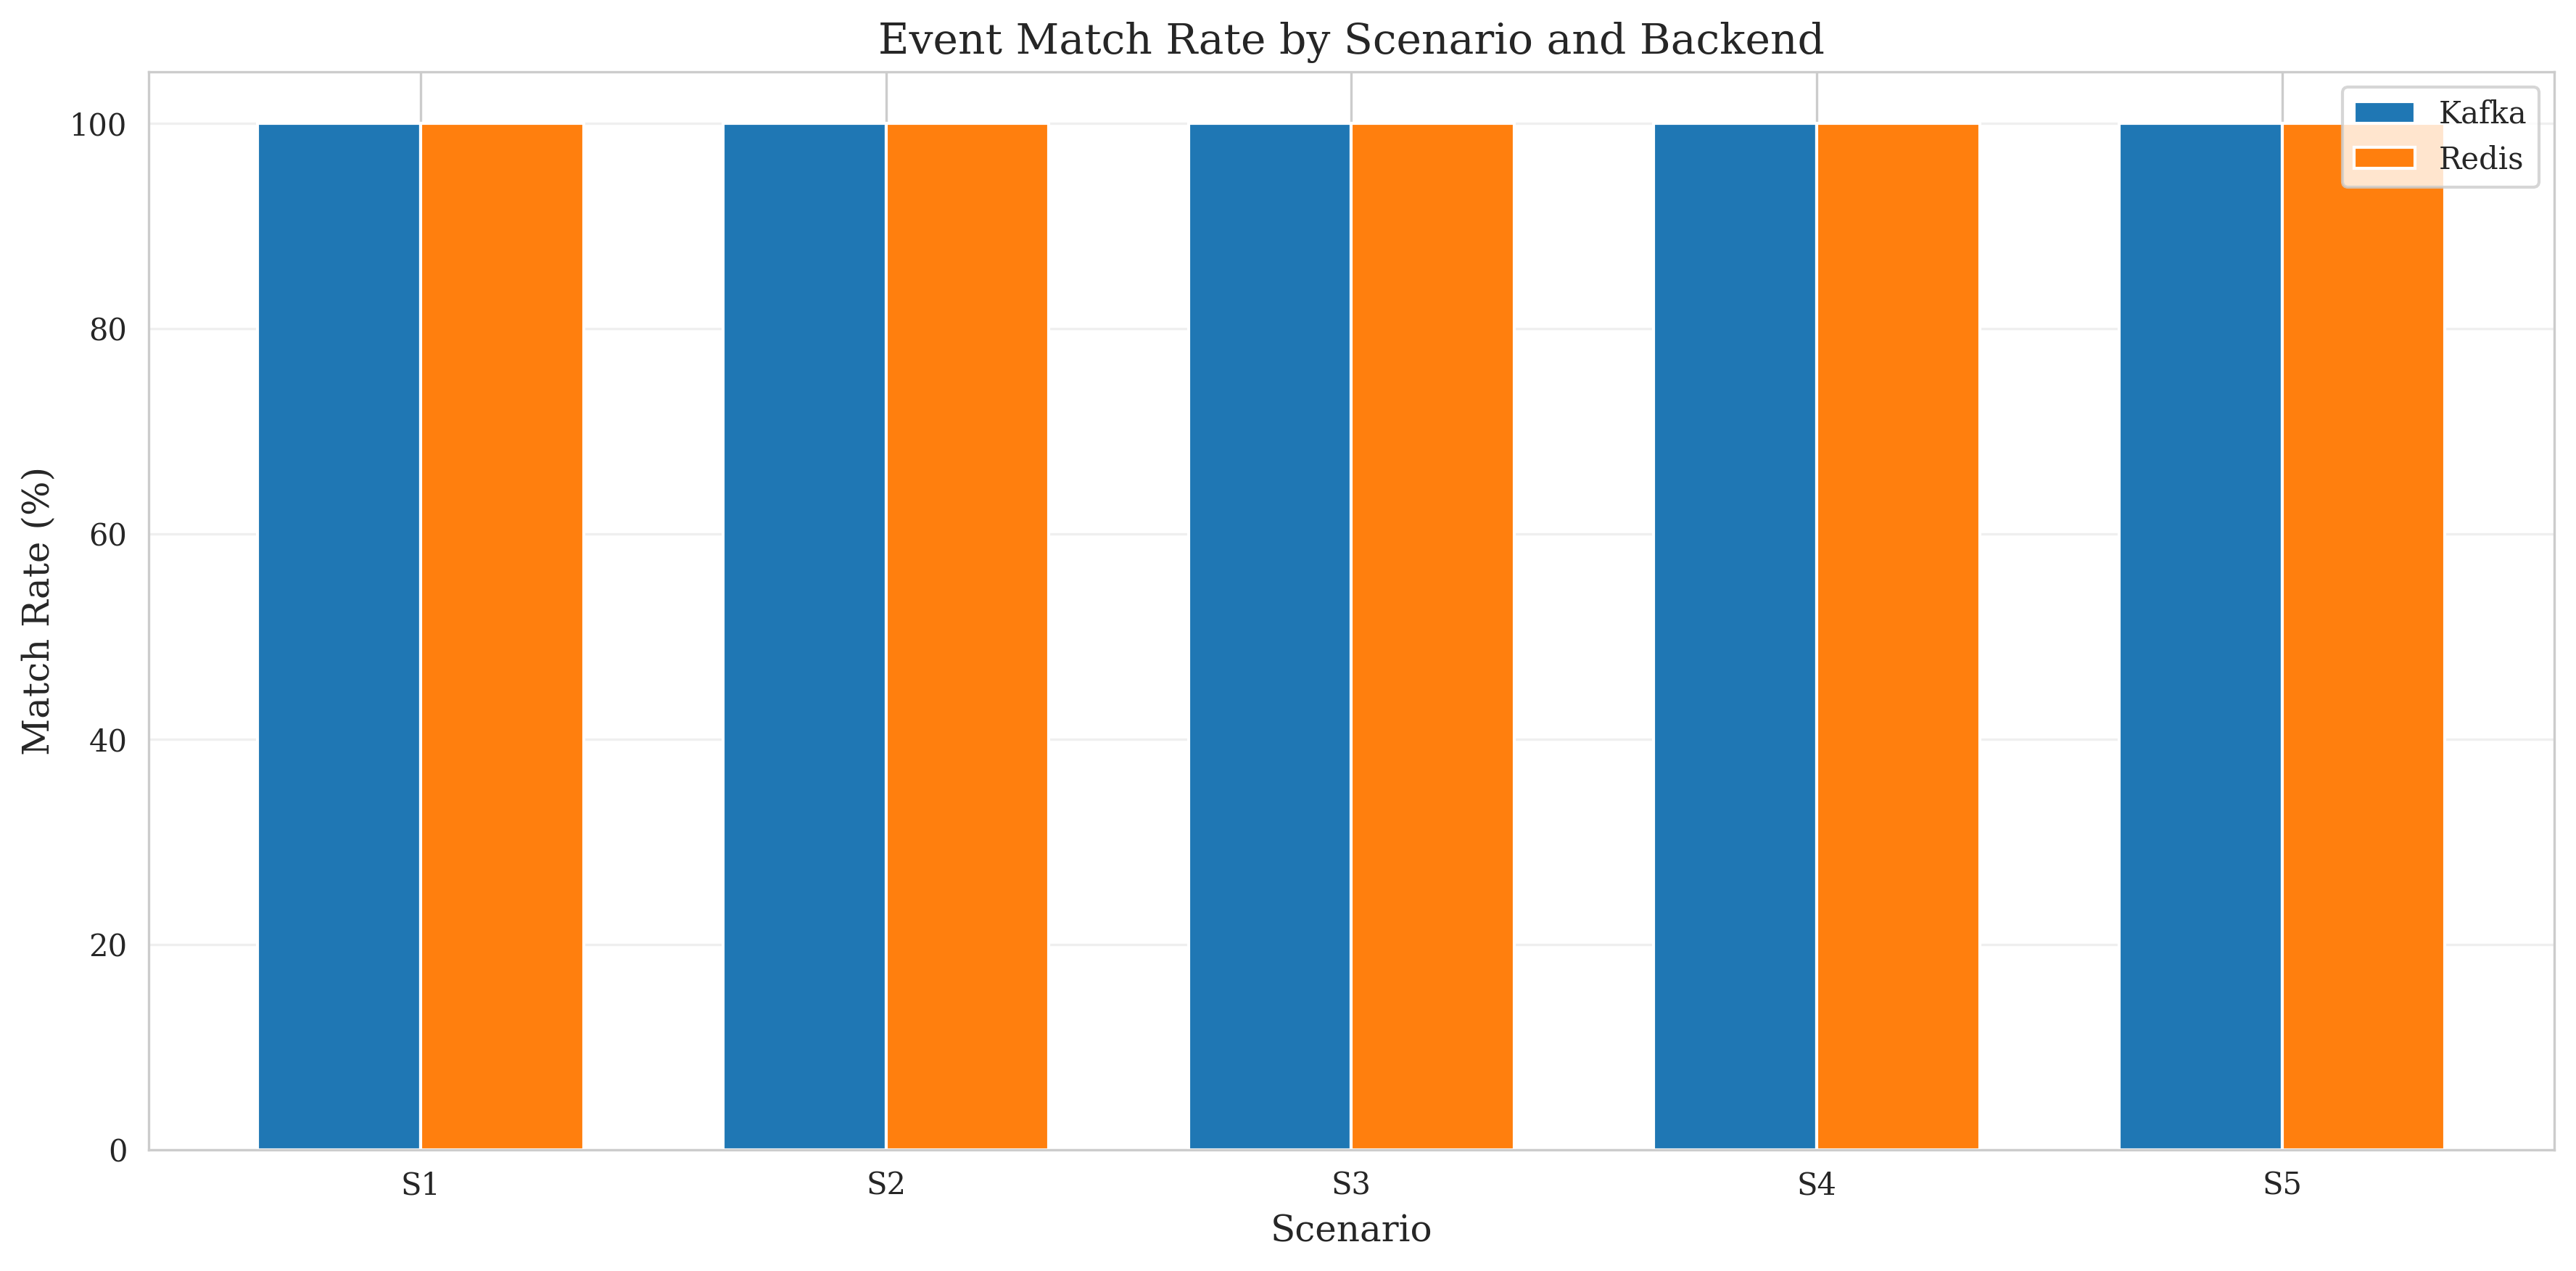
\includegraphics[width=0.8\textwidth]{docs/results/concurrency_sweep_20260613/match_rate_bars.png}
\caption{Event Match Rate by Scenario and Backend. All configurations achieve 100 percent match rates.}
\label{fig:matchrate}
\end{figure}

Key Results:
\begin{itemize}
\item Redis consistently achieves 40-55 percent lower TTI than Kafka across all scenarios
\item TTI remains stable across concurrency levels N=5, 10, 20 for both backends
\item All configurations achieve 100 percent event match rates
\item All performance differences are statistically significant (p < 0.001)
\end{itemize}

\section{Discussion}
\label{sec:discussion}
Redis 40-55 percent latency advantage attributed to: in-memory processing, efficient RESP protocol, minimal network hops, no batching overhead.

Both systems scale well to 20+ concurrent feeds.

Limitations: Single broker config, small message sizes, no fault tolerance testing.

\section{Conclusion}
\label{sec:conclusion}
This study presents comprehensive benchmarks comparing Apache Kafka and Redis Streams. 40,660 events, 250 runs, five scenarios, three concurrency levels.

Key findings:
\begin{enumerate}
\item Redis achieves 40-55 percent lower TTI than Kafka across all scenarios (p < 0.001)
\item Both systems scale excellently (stable TTI across N=5,10,20)
\item Both maintain 100 percent event match rates
\item Redis advantage consistent across all percentiles
\end{enumerate}

For low-latency sports analytics, Redis Streams provides clear advantage.

\end{document}
